\section{Struktur}

Dette pattern består af 2 vitale dele, Read siden og Write siden, Disse 2 dele, gør at patternet kan effektivt skrive eller læse til en data store. Princippet er at disse delen er Ren (Pure) og altså kun gør det som den er sat til. Write siden skriver kun til Datastore og returnere ikke nogen form for tilstand tilbage. Read siden mutere ikke data, men returnere kun Data. Disse handlinger er gjort igennem Commands og Queries.

\subsection{Generelt}

\begin{figure}[H]
	\center
	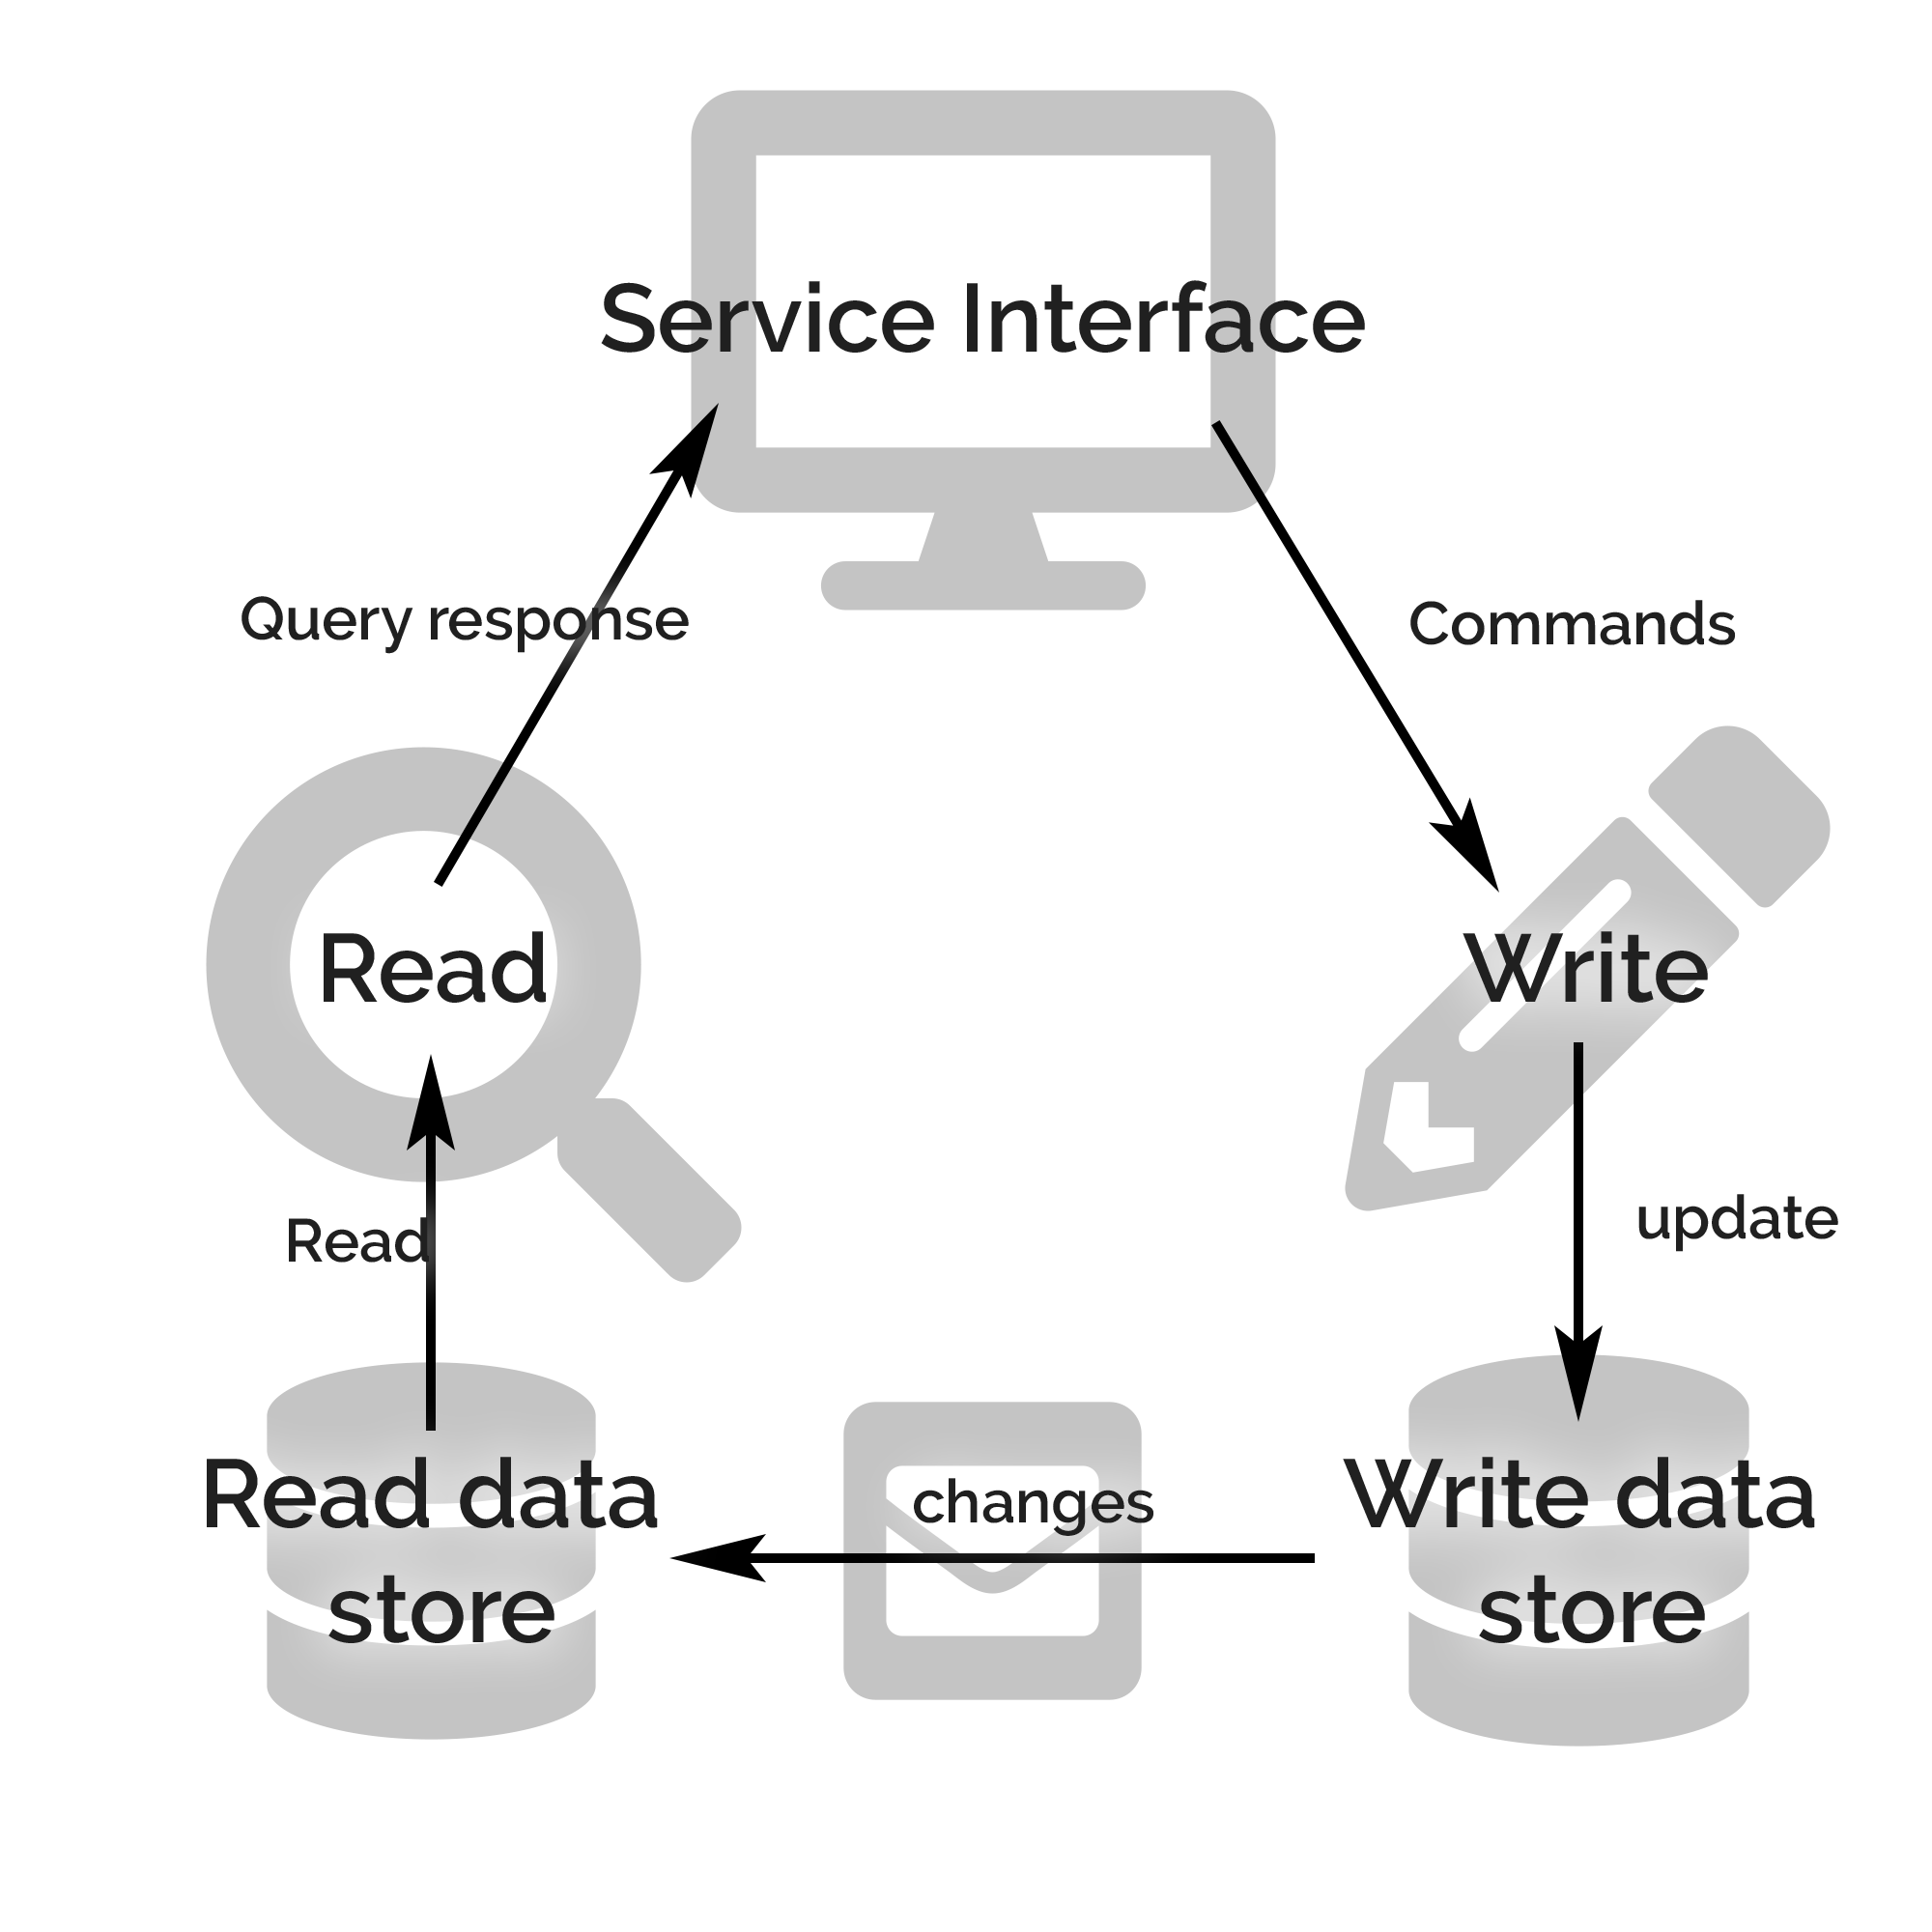
\includegraphics[width=0.7\textwidth]{CQRS-Model.png}
	\caption{Simpel CQRS med Read og Write}
	\label{fig:cqrs-model}
\end{figure}

\textit{``CQRS is simply the creation of two objects where there was previously only one. The separation occurs based upon whether the methods are a command or a query'' - Greg Young}

Generelt består CQRS af Commands og Query reponses samt Events. Commands rejser events når de bliver oprettet og gør det muligt at opdatere Read siden, med en successful transaktion.

Et scenarie der kan opstå er: Service interface sender en Command, til at mutere en model f.eks. oprette, slette, redigere en model, dette Command bliver valideret og på først Write data store samt også sendt Read data store. Read data store, bliver nu opdateret med frisk data og nu opdateret med Write data store. I en anden instans kan Service interface anmode Read siden med et query om en model fra Read data, og ønske at modtage et stykke data. Read siden opretter nu en DTO og returnere den med det ønskede data. 
\subsection{Read}

Read siden består Queries, hvor andre modeller kan anmode om DTO'er (Data Transfer Objects) Dette gør det let at hente data, næsten direkte fra Read data store, som næsten altid er opdateret af Write siden, Read data store, opfylder dog ikke \textit{Consistency} princippet, men nærmere \textit{Eventually Consistent} som gør at systemet skal tage høje for at der kan være samhørighedsproblemer på dataen. 
\subsection{Write}

Write siden består af Commands som kan mutere de modeller som findes i domain modellerne. 



